%!TEX root = ../book.tex
\chapter{Actuators}

The first part of this book has been concerned with different mechanisms, helping us understand how robots look like and how they move. We have then learned how robots can get information about their internal states and the world around them. We will conclude this part by introducing the devices that allow to turn energy into rotation and translation. We generally call such devices \textsl{actuators}\index{Actuators}. The goals of this chapter are to:

\begin{itemize}
\item provide a general overview over the different types of actuators and what their advantages and drawbacks are;
\item provide an appreciation of the systems challenges that come with any chosen actuator technology;
\item provide the basis and reference for further study.
\end{itemize}

\section{Electric motors}

Due to the dominance of rolling robots, the electric motor \cite{hughes2019electric} is among the most popular actuators. Electric motors come in different variations, starting with stepper and DC motors to servo and so-called ``brushless'' DC motors. Except for the stepper motor, which uses large electromagnets to rotate an internal spindle by a few degrees every time, the physics of the electrical motor requires it to revolve at very high speeds (multiple thousand rotations per minute). Therefore, electric motors are almost always used in conjunction with so-called reduction gears tasked with reducing their rotational speed and increasing their torque, i.e. the rotational force that the motor exerts to rotate about its axis.
Torques are indeed one of the most basic control commands that may be issued to control a motor (i.e., the lowest-level): a notion of joint torque was introduced in \cref{sec:forces:statics} and is generally employed when controlling a robot at the static\index{Statics} or dynamic\index{Dynamic} levels of abstraction.
In order to be able to measure the number of revolutions and the axis' position, motors are also often combined with rotary encoders (Section \ref{sec:sensors:encoders}). Motors that combine an electric motor with a gear-box, encoder, and controller to move toward desired position are known as servo motors, and are popular among hobbyists.

\subsection{AC and DC motors}

Electric motors turn electric energy into kinetic energy via electromagnetism. More specifically, an electric current running through a wire creates a circular magnetic field around the wire due to Ampere's law. This effect can be amplified by winding the wire into a coil. Due to the coil shape, the magnetic fields of all wires superimpose and create a strong magnetic field in the center of the coil. This field can be used to magnetize a ferromagnetic material such as iron, which in turn amplifies the magnetic field. The resulting \textsl{magnetomotive force} (MMF)\index{Magnetomotive force}\index{MMF---magnetomotive force} is directly proportional to the number of windings of the coil and the current running through it.

\subsubsection{AC motors}

In an AC motor, an electromagnetic coil is usually paired with a permanent magnet. As magnets of opposite polarity repel each other, this effect can be used to create motion. In its simplest form, an electric motor consists of a simple coil that can spin between two permanent magnets, one oriented with its south pole to the center, the other with its north pole (Figure \ref{fig:motor}, \emph{a}). Attaching a shaft to the central coil would then allow to turn a wheel, for example. The turning part with the shaft is known as the \textsl{rotor}\index{Rotor}, whereas the static part is known as the \textsl{stator}\index{Stator}. When running an electric current in the coil, the iron core will get magnetized: its north pole will then be attracted by the south pole of one magnet in the stator and repelled by the north pole of the other permanent magnet in the stator, while the opposite will happen to its south pole.

In order for this simple motor to not get stuck in its new configuration, we will need to swap the direction of the rotor's magnetic field. This can be achieved by swapping the direction of the current running through the coil. This happens by itself when using so-called \textsl{alternating current}\index{Alternating Current}, or \textsl{AC}\index{Alternating Current (AC)}. AC is commonly used in the power-grid, where the direction of current changes with a frequency of $50$ or $60$ Hz. In this case, the speed of the motor depends on the frequency of the AC, whereas its maximum torque is given by its current.

AC motors exist in different forms, often using multiple coils in parallel pairs to create smoother motions. Some motor designs also place the permanent magnets onto the rotor and coils on the outside. However, whatever the design is, the basic principles remain the same.

\subsubsection{DC motors}

As the speed of an AC motor is constant, it is mostly used in heavy industrial applications. An alternative design is to generate the desired switch in directionality by a so-called \textsl{commutator}\index{commutator} (Figure \ref{fig:motor}, \emph{b}). This allows running the motor with what is known as \textsl{direct current}\index{Direct Current}, or \textsl{DC}\index{Direct Current (DC)}, in which the direction of current does not change. DC is what is commonly available from batteries or from a ``wall wart'', that turns AC into DC by means of a transformer and a rectifier.

\begin{figure}
\centering
    % 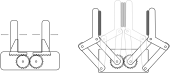
\includegraphics[width=\columnwidth]{figs/gripper-2-dof}
    \def\svgwidth{\textwidth}
    \import{./figs/}{motor.pdf_tex}
    \caption{Left: A simple motor consisting of a coil and two permanent magnets. In it's current configuration, the electromagnetic force will result in the coil to turn 180 degrees. Right: A simple commutator, which will switch the direction of the current and therefore of the magnetic field as the coil rotates.}\label{fig:motor}
\end{figure}

The commutator now provides positive and negative voltage at a series of interleaving pads. These can be placed along the circumference of the stator and provide power to the rotor coil via metal brushes attached to the shaft. By this, the central coil will receive power at the right polarity no matter where it is. As with the AC motor, there exist multiple designs using pairs of parallel coils, various number of brushes, and commutators mounted either in the stator or the rotor.

Such a motor can now turn at arbitrary speeds and will become faster and faster, only limited by friction and torque applied to its shaft. Its speed is therefore proportional to the voltage that is applied, whereas its torque is limited by the maximum current that is provided.

Electric DC motors are widely used in robotics, but suffer from low efficiency due to the friction of the brushes and their wear-and-tear.

\subsection{Stepper motor}

Even when using more than one coil and multiple pairs of permanent magnets, it is difficult to precisely control the angular position of a DC motor shaft. Although the rotation can be geared down by factors of hundreds or even thousands, the motor itself usually spins in the order of thousands of times per minute---also known as ``rotations per minute'' or RPM\index{Rotations per minute}\index{Rotations per minute (RPM)}.
%
A solution to this problem is the \textsl{stepper motor}\index{Stepper motor} that---in its simplest form---uses a ferromagnetic rotary wheel with a fixed number of teeth as its stator. Coils in its stator can attract these teeth, creating a small rotation of a few degrees when the teeth in the rotor and stator-coil align. To precisely control this effect, the ferromagnetic material in the coil also has a teeth pattern. Selectively turning pairs of coils on and off will allow the motor shaft to turn at a fixed number of degrees (in the order of one degree or less). For example, a stepper motor that turns 3.6 degrees per step will require 100 steps for a complete revolution.

The required voltage pattern is usually generated by a microcontroller. A stepper motor with four phases, that is four sets of coils in the inside, requires four electrical signals that are carefully interleaved. That is, the first wire is on for a set amount of time while the other three are off, then the second, the third, and the fourth.
Here, the period (i.e. the length) of this signal determines the stepper motor's speed, whereas the maximum current determines its holding torque.
There exists a variety of low-cost integrated circuits (ICs) that generate this pattern, reducing the microcontroller's task to simply sending a single bit for every step and another for the desired direction.

The advantage of this approach is that stepper motors usually do not require gears or encoders (as one can simply count the steps being sent), making them attractive as drivers for small differential wheel robots or grippers. Stepper motors are usually much more expensive and bulky than their DC counterparts.

\subsection{Brushless DC motor}\label{sec:brushlessDC}

As the alternating current patterns are generated by electronics, the stepper motor does not require brushes to commutate and is therefore much more efficient. The advent of microelectronics in the Seventies has enabled to generate driving patterns at the speeds required by conventional DC motors (thousands of RPMs), which has led to the \textsl{brushless DC motor}\index{brushless DC motor}. The brushless DC motor indeed resembles a stepper motor, but can operate with much smaller coils as its torque results from the kinetic energy of rotating at high speeds. In order to improve control, brushless DC motors either use encoders, a Hall effect sensor, or small changes in current that result from the dynamo effect in the currently unused coils, to measure the current position of the rotor within the stator. Sensing and control of a brushless DC motor is involved and usually provided by purposely designed solid-state electronic devices.

Unlike a brushed DC motor, whose brushes induce friction, the maximum speed of a brushless DC motor is mostly limited by heat, which is a byproduct of running electric current through its coils. Due to the absence of friction, brushless DC motors are far more efficient than their brushed counterparts and can provide equivalent speed and torque at a smaller form factor and lower weight.

The performance of electric motors has been further boosted by the discovery of rare earth magnets such as neodymium in the Eighties, allowing motors to exert even more torque at smaller weight and using lesser current. Together, these advances have led to a renaissance of electric cars and, together with solid-state IMUs (Section \ref{sec:gyroscopes}), enabled small-scale drones.

\subsection{Servo motor}

To be useful in a robotic system, electric motors usually require gears, an encoder, and control electronics. Modules that package these components into a convenient form-factor are known as \textsl{servo motors}\index{servo motors}.

Servo motors have been classically used in remote controlled (RC) cars to provide a simple actuator to steer a car or move the flaps of an airplane. A simple digital signal was used to set the servo angle, usually in the range of 360 degrees or less, which was then held by the integrated electronics. More recently, a new class of digital servo motors have emerged that allows to not only control the angle, but set the speed at which the servo moves as well as the maximum current (and thereby torque), as well as read information such as actual angle, temperature and other operational parameters.

Due to their built-in gear reduction, servo motors are usually not suitable in the drivetrain of mobile platforms, but have become increasingly prominent to drive the joints of simple manipulating arms, articulated hands and grippers.
%
A special kind of servo motor is the \textsl{linear actuator}\index{linear actuator}. Here, a (brush-less) DC motor is driving a spindle that turns rotation into translation. Linear servo motors are available with a wide range of protocols and with or without built-in encoders that provide position feedback.

\subsection{Motor controllers}

Designing the power electronics that turn digital information into precisely controlled voltage and currents is particularly challenging. Transistors are used to turn low-power control signals from a micro-controller into high powered ones, while regulating the voltage is achieved by switching DC power on and off at very high frequency (tens of kHz) and smoothing the signal using a combination of capacitors and coils. Diodes are used to ground the reverse voltage that arises from demagnetizing coils. As peak-loads of tens of Amperes will already arise in smaller systems such as remote controlled cars, designing a motor controller is very involved and usually limited to a specific operational range.

The biggest challenge in selecting appropriate circuits for motor drivers is selecting a circuit that can not only accommodate the voltage ($U$) and current ($I$) requirements, but can actually handle the overall energy ($P=UI$). Here, the first hurdle is to provide the desired supply voltage. As it is difficult to convert supply voltages without loss (in particular when the required current is large), voltage requirements of the main driving motors often determine the operating voltage of the overall power system.

A second hurdle is that there is nothing like loss-less energy switching. In particular, all power transistors have an internal resistance ($R$). Given $P=I^2R$, already small resistances generate substantial heat. Dissipating the resulting heat can quickly become a major problem; typically, this is not part of an off-the-shelf motor control solution, but it represents a mechanical design problem in and of itself. A standard approach is to use the (metal) robot chassis to dissipate heat, but sometimes active cooling using a fan is necessary. For more details on designing power electronics for a variety of electric motors, the reader may refer to \cite{hughes2019electric}.

\section{Hydraulic and pneumatic actuators}

Another popular class of actuators, in particular for legged robots, are linear actuators, that might exist in electric, pneumatic or hydraulic form.

\subsection{Hydraulic actuators}

Hydraulic actuators, mostly in the form of pistons, are well known from construction machines and other heavy equipment. Hydraulics usually exceed the forces electric motors can generate and are in a different ballpark as far as size is concerned. That is, the smallest available hydraulic actuators are orders of magnitude larger (in the order of tens of centimeters) than the smallest DC motors (in the order of millimeters). However, they are relevant for larger bipedal and quadrupedal platforms, where they are often used in conjunction with electric motors.

Hydraulic actuators require a tank with pressurized liquid and a compressor pump (which is again driven by a DC motor). The liquid is pressurized using a gas, and released into the actuators via solenoid valves. A second solenoid valve is used to let the liquid escape the actuator. The compressor is then pumping the liquid back into the tank. Here, the gas in the tank acts as a buffer allowing the system to release a burst of energy, which then needs to be slowly restored by the compressor. As the performance of a hydraulic system is strongly related to its mechanical properties such as size and pressure of the tank, diameter of the tubes connecting the components, and dimensions of the valve, hydraulic systems have a narrower operational range than electric motors, which allow a higher variation of forces and speeds.
However, they are costly to maintain, difficult to control, and they are usually characterized by a low bandwidth: that is, they will never be as reactive as electric motors, and they might be infeasible in human-populated environments where speed of reaction is paramount for safety considerations (\cref{sec:actuators:safety}).

\subsection{Pneumatic actuators and soft robotics}

The principles of fluid-based (hydraulic) actuators also extend to operation by air. Pneumatic systems also require a compressor, a tank, and a set of valves to direct the flow of air. As air is orders of magnitudes more compressible than a liquid, pneumatic systems are not well suited to translate large forces, but are lightweight and available in much smaller form factors than hydraulic systems. For example, solenoid valves can be as small as a few millimeters, allowing to construct intricate mechanisms such as realistically-sized robotic fish \cite{katzschmann2018exploration} or robotic hands \cite{deimel2016novel}.

In addition to pistons and other actuators available for hydraulic systems, pneumatic actuators can be designed in arbitrary form factors, allowing the designer to turn air pressure into almost any desired bending or torsional movement. These actuators usually consist of a flexible rubber material with an internal cavity that can be filled with air. Materials such as fabrics that are stiff in one dimension (when pulling), but flexible in another (when bending), are used to direct the force of the incoming air into a desired direction, resulting into the actuator bending or twisting in a desired way \cite{polygerinos2017soft}. Please note that soft actuators are \textsl{not} balloons. While balloons change their volume as they are inflated, a change of volume is considered a failure mode in a soft robotic actuator and, ideally, all energy should directly convert into motion.

As soft actuators are flexible, they break with the tradition of kinematics for rigid robots introduced in \cref{chap:kinematics}. From a kinematic perspective, an ideal, fully soft robot can be modeled as a platform with an infinite number of mechanical degrees of freedom!
However, although their complex mechanics makes modeling and control more difficult, soft robotics opens up an entirely new spectrum of robot capabilities; for example, it is possible to design non-traditional kinematics that more resemble the motion of animals than those of machines. This also allows to employ control strategies that rely on the mechanism to give in, also known as \textsl{compliance}\index{Compliance}, a concept briefly introduced in Section \ref{sec:simplegrasp} on robotic grasping, and enabled by force control (\cref{ch:forces}).


%\section{Other actuators}
% Finally, there exist a wide array of specialty actuators such as Shape-Memory Alloys, Electroactive Polymers or Piezo-elements, which often allow for extreme miniaturization, but do not provide attractive energy-to-force ratios and are difficult to control.

\section{Safety considerations}\label{sec:actuators:safety}
Which actuator system is the best choice is also driven by safety considerations. We distinguish \textsl{active} and \textsl{passive} safety. Active safety is the ability to control the actuator sufficiently to avoid it to do harm---e.g. by squeezing a person's finger or limb, or damaging infrastructure in the environment. The class of \textsl{collaborative robots}\index{Collaborative robot}\index{Collaborative Robot}\index{Cobot} achieves that by limiting the torque a robot can achieve through control. %, an approach known as \textsl{soft robotics} \cite{albu2008soft}, albeit unrelated to soft pneumatic actuators that derive additional safety properties from compliance.
Controlling torque can be accomplished by measuring and regulating the current that is used at any given actuators, and employing a suitable low-level dynamical model of the motor that relates operating current with motor torque. By comparing the joint torques needed to perform a task (see \cref{ch:forces}) with the currents actually flowing through the motors, a robot can detect whether it is about to exert a (potentially harmful) force or torque on the external world.
This usually requires estimating the approximate weight of the robot's payload. A better (but more expensive) way to control torque is to measure it at each joint by means of load cells (see \cref{chap:sensors}). Using actual sensors to measure forces and torques actually allows to extend this method to other actuation systems, not limited to electrical motors.

Passive safety is the ability to maintain a robot's safety even in the absence of control. This can be achieved by cushioning a robot, using actuators that ``give in'' at a lower force than can do harm, such as pneumatic actuators, or by coupling the motor with an elastic element. In such \textsl{series elastic actuators}\index{Series Elastic Actuators}, power is not directly transmitted via a motor shaft, but indirectly through a spring. In addition to doubling as a force/torque sensor (see also \cref{chap:sensors}), this limits the maximum force such an actuator can exert and reduces the precision of any high-level controller.

An important failure mode that can only be addressed by a passive safety mechanism is \textsl{power failure}\index{Power failure}. In the absence of power, a mobile robot might keep driving (based on inertia) and hit an object, a humanoid robot might collapse onto itself, and a gripper might let a heavy (or sharp) payload fall. These problems can be addressed by always-on breaking mechanisms that engage in the absence of power or by using gear ratios that are so high that the overall mechanism is not back-driveable.

\section*{Take-home lessons}
\begin{itemize}
\item There exist an almost limit-less repertoire of techniques to turn energy into motion, many of which have been explored to create robots, with the electric motor remaining the dominant actuator in small-scale robotic systems.
\item What makes a good actuator is not only determined by its efficiency with respect to the available energy source, but also in how far its position, velocity, and torque can be measured to enable accurate and precise control.
\item A robot's safety is determined not only by the choice of actuator, but also by the control system around it.
\end{itemize}



\section*{Exercises}\small
\begin{enumerate}
\item You are designing a robotic arm. Your goal is to maximize strength, while minimizing weight. Which kind of electric motor do you chose and why?
\item You are designing a gantry system for a 3D printer that can move the print head left, right, up and down.
\begin{enumerate}
\item What kind of electric motor is your preferred choice and why?
\item The motor you selected requires 5V and up to 1A. Select an appropriate driver board from an online vendor.
\item What additional components would you need to realize the gantry with a brushless DC motor?
\end{enumerate}
\item A motor you selected for the shoulder joint of a robotic arm is too weak and stalls under load. Assuming power is provided uninterrupted, what will eventually lead to permanent damage?
\item The key component in a motor controller has a so-called ON-resistance of 0.2$\Omega$. Your motor requires 10A at average load.
\begin{enumerate}
\item What is the power dissipated at heat?
\item Search the internet for thermal heat sinks. What are the key quantities to look out for here?
\end{enumerate}
\item Compare the parallel jaw gripper with a 2-bar linkage gripper. Discuss their safety properties in case of power failure.
\item The end-effector of a ``soft'' robotic arm is hitting an object with 3 m/s. Discuss its safety when compared with a conventional robotic arm and state the assumptions you are making. 
\end{enumerate}\normalsize
